% All Memory Is Local — ICLR 2027 submission version
\documentclass{article}
\usepackage{iclr2027_conference,times}

% Math and formatting packages
\usepackage{amsmath,amssymb,amsthm}
\usepackage{graphicx,booktabs,xcolor,microtype}
\usepackage{hyperref}
\usepackage{url}

% Theorem environments
\newtheorem{proposition}{Proposition}
\newtheorem{remark}{Remark}

% Load auto-generated numbers
\newcommand{\baseAccZero}{0.9}
\newcommand{\basePplZero}{3510}
\newcommand{\baseAccFive}{1.0}
\newcommand{\basePplFive}{3437}
\newcommand{\baseAccFifteen}{1.0}
\newcommand{\basePplFifteen}{3451}
\newcommand{\baseAccForty}{1.0}
\newcommand{\basePplForty}{3556}
\newcommand{\persistAccZero}{7.1}
\newcommand{\persistPplZero}{398}
\newcommand{\persistAccFive}{2.5}
\newcommand{\persistPplFive}{678}
\newcommand{\persistAccFifteen}{1.9}
\newcommand{\persistPplFifteen}{825}
\newcommand{\persistAccForty}{1.7}
\newcommand{\persistPplForty}{934}
\newcommand{\sessionAccZero}{4.6}
\newcommand{\sessionPplZero}{1229}
\newcommand{\sessionAccFive}{1.0}
\newcommand{\sessionPplFive}{3437}
\newcommand{\sessionAccFifteen}{1.0}
\newcommand{\sessionPplFifteen}{3451}
\newcommand{\sessionAccForty}{1.0}
\newcommand{\sessionPplForty}{3556}
\newcommand{\consistencyAccZero}{8.5}
\newcommand{\consistencyPplZero}{358}
\newcommand{\consistencyAccFive}{3.6}
\newcommand{\consistencyPplFive}{578}
\newcommand{\consistencyAccFifteen}{2.2}
\newcommand{\consistencyPplFifteen}{747}
\newcommand{\consistencyAccForty}{1.7}
\newcommand{\consistencyPplForty}{873}
\newcommand{\randomAccZero}{7.3}
\newcommand{\randomPplZero}{401}
\newcommand{\randomAccFive}{2.6}
\newcommand{\randomPplFive}{669}
\newcommand{\randomAccFifteen}{2.0}
\newcommand{\randomPplFifteen}{823}
\newcommand{\randomAccForty}{1.8}
\newcommand{\randomPplForty}{925}
\newcommand{\persistExcessLagZero}{6.2}
\newcommand{\persistExcessLagZeroCI}{[5.0,\,7.5]}
\newcommand{\persistExcessLagForty}{0.67}
\newcommand{\persistExcessLagFortyCI}{[0.29,\,1.05]}
\newcommand{\persistExcessLagFive}{1.6}
\newcommand{\persistExcessLagFifteen}{0.9}
\newcommand{\foldLagZero}{7.6}
\newcommand{\crZero}{1.22}
\newcommand{\crZeroCI}{[0.59,\,1.91]}
\newcommand{\crFive}{1.00}
\newcommand{\crFiveCI}{[0.52,\,1.52]}
\newcommand{\crFifteen}{0.21}
\newcommand{\crForty}{-0.11}
\newcommand{\rpZero}{0.16}
\newcommand{\rpZeroCI}{[-0.18,\,0.51]}
\newcommand{\spZero}{-2.5}
\newcommand{\spZeroCI}{[-3.4,\,-1.8]}
\newcommand{\spForty}{-0.7}
\newcommand{\sessionCapture}{60}
\newcommand{\sessionCaptureMin}{45}
\newcommand{\sessionCaptureMax}{72}
\newcommand{\sessionLogCapture}{48}
\newcommand{\freshTransfer}{0.35}
\newcommand{\freshTransferCI}{[-0.14,\,0.91]}
\newcommand{\freshCR}{0.07}
\newcommand{\freshCRCI}{[-0.38,\,0.52]}
\newcommand{\crSmallZero}{0.64}
\newcommand{\crSmallZeroCI}{[-0.14,\,1.62]}
\newcommand{\crSmallFive}{0.69}
\newcommand{\crSmallFiveCI}{[-0.09,\,1.55]}
\newcommand{\persistSmallExcessZero}{7.9}
\newcommand{\persistSmallExcessForty}{0.16}
\newcommand{\persistSmallExcessFortyCI}{[-0.33,\,0.72]}
\newcommand{\crLargeZero}{1.56}
\newcommand{\crLargeZeroCI}{[0.57,\,2.63]}
\newcommand{\crLargeFive}{1.74}
\newcommand{\crLargeFiveCI}{[0.77,\,2.90]}
\newcommand{\persistLargeExcessZero}{7.7}
\newcommand{\persistLargeExcessForty}{0.45}
\newcommand{\persistLargeExcessFortyCI}{[-0.27,\,1.30]}
\newcommand{\normTwo}{0.27}
\newcommand{\normThree}{0.25}
\newcommand{\normFour}{0.21}
\newcommand{\taxHSRaw}{-3.0}
\newcommand{\taxHSNorm}{-3.3}
\newcommand{\taxPIQARaw}{-2.7}
\newcommand{\taxPIQANorm}{-2.5}
\newcommand{\taxARCERaw}{+0.1}
\newcommand{\taxARCENorm}{+3.7}
\newcommand{\taxARCCRaw}{+1.5}
\newcommand{\taxARCCNorm}{+2.0}
\newcommand{\taxWGRaw}{-0.5}
\newcommand{\taxWGNorm}{-0.5}
\newcommand{\eThreeStreamZero}{-1.23}
\newcommand{\eThreeStreamForty}{-1.07}
\newcommand{\eThreeFresh}{-1.17}
\newcommand{\eThreeFreshCI}{[-1.30,\,-1.05]}
\newcommand{\eThreeShare}{96}
\newcommand{\eThreeCRZero}{-0.10}
\newcommand{\eThreeCRZeroCI}{[-0.14,\,-0.07]}
\newcommand{\eThreeCRForty}{-0.19}
\newcommand{\eThreeFreshCR}{-0.17}
% P(L) = session-specific persistence = streamed excess - fresh transfer
% Combined CIs from independent bootstraps over streamed and fresh sessions
\newcommand{\memZero}{5.8}      \newcommand{\memZeroCI}{[4.5,\,7.3]}
\newcommand{\memFive}{1.2}      \newcommand{\memFiveCI}{[0.5,\,2.0]}
\newcommand{\memFifteen}{0.6}   \newcommand{\memFifteenCI}{[-0.1,\,1.2]}
\newcommand{\memForty}{0.3}     \newcommand{\memFortyCI}{[-0.4,\,1.0]}

\newcommand{\nRepos}{180}
\newcommand{\nHoldout}{124}
\newcommand{\nFresh}{43}
\newcommand{\nESessions}{203}
\newcommand{\nXfileTargets}{2045}


% Custom commands
\newcommand{\pt}{\,\mathrm{pt}}

% Anonymous submission
\title{All Memory Is Local:\\Measuring the Horizon of Persistent Test-Time Training}
\author{Anonymous authors}

%\iclrfinalcopy % Uncomment for camera-ready version

\begin{document}
\maketitle

\begin{abstract}
Test-time training (TTT) lets a language model update a small set of fast weights as it reads. The drop-in methods considered here reset those weights at document boundaries, so nothing carries across documents. When the reset is removed, the model recalls symbols from earlier documents well after they have left the context, which looks like persistent memory. We ask how much of this signal is memory. Delayed recall has at least three other sources: information the model already had (pre-training contamination, in-context copying, synthetic vocabularies shared across sessions), properties of the evaluation (scoring order, length-normalized accuracy), and adaptation to the stream as a whole. We build a protocol, Streaming-TTT, that separates them: per-session obfuscated vocabularies, first-mention targets, fixed-lag re-scoring, and a control of sessions that were never streamed. On 180 code repositories and 200 prose sessions with Qwen3 models from 0.6B to 4B, persistence raises first-mention recall to \foldLagZero\ times the frozen model's immediately after a session, but the estimated session-specific component falls by about four fifths within five sessions; by lag~15 what remains cannot be distinguished from the gain on never-streamed sessions. A linear-interference model predicts that this decay depends on subsequent write mass rather than on the learning rate, and the measured curves collapse accordingly. Resetting at session boundaries keeps \sessionCapture\% of the immediate benefit and avoids the general-capability cost that unrestricted persistence incurs. In this setting, delayed recall alone did not establish persistent memory; the relevant quantity is what remains after adaptation is subtracted.
\end{abstract}

\section{Introduction}
Test-time training adapts a language model by updating fast weights, typically the MLP down-projections, as tokens arrive. It appears both in architectures trained for it (Titans, \citealp{behrouz2025titans}; LaCT, \citealp{zhang2025lact}; TTT-E2E, \citealp{tandon2025ttte2e}) and in drop-in variants applied to pretrained models (In-Place TTT, \citealp{feng2026inplace}; TTT-NTP, \citealp{ouyang2026tttntp}). The drop-in methods considered here reset the fast weights at document boundaries.

Real workloads are streams: a coding assistant reads one repository file after another; an enterprise assistant reads one organization's documents for months. If the reset is simply removed, the model does something that looks like remembering. It recalls identifiers defined in a file it read several files ago, long after that file has left the context window. This paper asks how much of that signal is memory, and how far it reaches.

The question is harder than it sounds, because delayed recall has other sources. Some of the information was never learned at test time at all: on unmodified public repositories, a frozen model already recalls 38.1\% of cross-file identifiers, and every mention of a symbol after the first can be copied from context. Some of the signal comes from the evaluation rather than the model: scoring a chunk after it has been written, or using length-normalized accuracy, both move the numbers. And some of it is adaptation to the stream as a whole rather than to any particular session; on prose, this component accounts for \eThreeShare\% of the apparent likelihood gain. These sources did not all become visible at the same stage of the study, and our protocol was refined as they did. Its final form (\S\ref{sec:protocol}) renames every session-defined symbol with a session-specific vocabulary, scores only first mentions, re-scores held-out documents at fixed lags after learning, and compares against sessions that were never streamed.

With these controls, the measurement gives a consistent picture across code and prose, with the same qualitative pattern across the model sizes we evaluate. Persistence raises first-mention recall to \foldLagZero\ times the frozen model's immediately after a session. The session-specific part of that gain falls by about four fifths within five sessions; by lag~15 the remaining excess ($\persistExcessLagFifteen\pt$) lies within the interval of the gain on never-streamed repositories ($\freshTransfer\pt$, CI \freshTransferCI), and by lag~40 the two coincide. The control therefore turns delayed recall into a measurement of session-specific retention. A linear-interference model (Prop.~\ref{prop:snr}) predicts that the decay depends on how much is written afterwards and not on the learning rate; curves at three learning rates collapse when normalized (Fig.~\ref{fig:collapse}). Unrestricted persistence also costs $2$--$3\pt$ on HellaSwag and PIQA. Resetting at session boundaries keeps \sessionCapture\% of the immediate benefit with no cross-session exposure. Finally, at equal write budget, gating writes by cross-document sign consistency beats random placement by about one point at lag~0; the effect is larger on larger models and disappears by lag~15.

Our contributions are: (1) a protocol for measuring persistent TTT that separates prior knowledge, evaluation effects, and stream adaptation from session-specific memory, with unit tests and a never-streamed control; (2) measurements on code and prose streams at three model sizes showing that session-specific memory decays within a few sessions and that the long-lag residual is not distinguishable from adaptation; (3) evidence that sign-consistency gating improves short-lag retrieval at equal write budget, with a larger effect on larger models.

\section{Related Work}
\textbf{TTT and fast weights.} Fast-weight memories date to \citet{schmidhuber1992fast} and \citet{ba2016fast}; linear attention is their modern form \citep{katharopoulos2020transformers,schlag2021linear}. Contemporary TTT instantiates them as inner-loop learners: TTT-Linear/MLP \citep{sun2024ttt}, LaCT \citep{zhang2025lact}, TTT-E2E \citep{tandon2025ttte2e}, Titans \citep{behrouz2025titans}, HOPE \citep{behrouz2025nested}, DeltaNet variants \citep{yang2024deltanet,yang2025gated}, and drop-in retrofits In-Place TTT \citep{feng2026inplace} and TTT-NTP \citep{ouyang2026tttntp}; single-input adaptation \citep{hardt2024tttnn,hubotter2025sift}. All reset per sequence or document, or require (meta-)training; none measures cross-session retention. We adopt In-Place TTT's fast-weight location and chunk-wise schedule; we vary only whether fast weights persist across documents.

\textbf{Continuous TTT inside episodes.} Agentic TTT \citep{agentic2026ttt} and TTT-Discover \citep{yuksekgonul2026discover} update continuously within one agent episode. Their stream is the model's own text; ours is an exogenous document stream across sessions.

\textbf{Context-to-weights persistence.} Temp-LoRA \citep{wang2024temlora}, StreamAdapter \citep{muhtar2024streamadapter}, InfiniteICL \citep{cao2025infiniteicl}, SCoL \citep{scol2026}, CaMeLS \citep{hu2023camels} and MAC \citep{tack2024mac} write context into parameters, several with meta-training, several noted to erode general capability. These works propose mechanisms; we contribute a measurement framework for the training-free case. Concurrently, \citet{persistentmem2026} compares trained latent memory banks attached to a frozen encoder--decoder under a cross-session forgetting curve; our object is the LM's own fast weights, training-free, with the lag protocol and controls of \S\ref{sec:protocol}.

\textbf{Continual test-time adaptation in vision.} CoTTA \citep{wang2022cotta}, EATA \citep{niu2022eata}, SAR \citep{niu2023sar} and Elastic TTT \citep{ma2026elastic} stabilize non-reset adaptation for classification and reconstruction, the latter two with Fisher penalties. We evaluate non-reset adaptation as one member of our policy family; these works do not measure recall as a function of lag.

\textbf{Memory theory.} Palimpsest models \citep{parisi1986memory}, cascade synapses \citep{fusi2005cascade} and \citet{benna2016computational} predict decay governed by subsequent write load, not time. Fig.~\ref{fig:collapse} tests this prediction on an LLM's fast weights. Our Fisher gate is a test-time analogue of importance weighting in EWC \citep{kirkpatrick2017ewc}, SI \citep{zenke2017si}, and MAS \citep{aljundi2018mas}; transfer metrics follow \citet{lopezpaz2017gem}.

\section{Persistent Test-Time Training}
\subsection{Setup}\label{sec:setup}
A pretrained causal LM processes an ordered stream of \emph{sessions} (files of one repository; sections of one article), each a sequence of \emph{documents}. Following In-Place TTT, the fast weights are the MLP down-projections, consistent with evidence that MLP layers store associations \citep{geva2021ffn,meng2022rome}: $W_{\mathrm{eff}} = W_{\mathrm{base}} + G_{\mathrm{slow}} + G_{\mathrm{fast}}$, both $G$ initialized to zero. Within a document, each chunk of $C{=}256$ tokens is first \emph{scored} under the current $W_{\mathrm{eff}}$ (all metrics are prequential: each chunk is scored before it is written, so no chunk is ever scored after the model has learned from it) and only then \emph{written}:
$\delta = \mathrm{clip}_{\pm m}(-\eta\,\nabla_{W}\mathcal{L}_{\mathrm{NTP}}(\text{chunk}))$, $G_{\mathrm{fast}} \mathrel{+}= \delta$.
No optimizer state is kept; the method is training-free and drop-in.

\subsection{What counts as persistence?}\label{sec:estimand}
Three quantities are easy to conflate. \emph{Within-session adaptation} is the gain on a session's held-out document scored immediately after the session (lag~0). \emph{Stream adaptation} is what the model has absorbed about the stream as a whole (vocabulary shape, domain style); we use the gain the final fast-weight state produces on sessions that were never streamed as an estimate of this quantity, since that gain cannot be memory of any particular session. \emph{Session-specific persistence} at lag $L$ is what is left of a session's gain, $L$ sessions after it was learned, once stream adaptation is accounted for. We estimate it as
\[
P(L) \;=\; \big[R_{\text{streamed}}(L) - R_{\text{frozen}}\big] \;-\; \big[R_{\text{fresh}} - R_{\text{frozen}}^{\text{fresh}}\big],
\]
where $R$ is first-mention recall (or, on prose, log-likelihood), each excess is taken against the frozen model on the same documents, and the second bracket is measured on never-streamed sessions with the state at the end of the stream. The first bracket alone is what a delayed-recall experiment reports; $P(L)$ is the quantity our conclusions are about. Intervals for $P(L)$ combine a session-clustered bootstrap over streamed sessions with an independent one over never-streamed sessions.

\subsection{A family of persistence policies}
At each document boundary $G_{\mathrm{slow}} \leftarrow \gamma G_{\mathrm{slow}} + \alpha \odot G_{\mathrm{fast}}$, $G_{\mathrm{fast}} \leftarrow 0$ unifies: \textbf{reset} ($\alpha{=}0$), \textbf{persist} ($\alpha{=}1,\gamma{=}1$), \textbf{decay} ($\gamma{<}1$), \textbf{consistency} ($\alpha=\Pi:=|\mathrm{EMA}_{\gamma_d}[\mathrm{sign}\,G_{\mathrm{fast}}]|$), \textbf{Fisher} ($\alpha=(1+\hat F/\mathrm{med}\,\hat F)^{-1}$, with $\hat F$ a within-document moving average of squared gradients), \textbf{surprise} (a scalar $\alpha$ from the document's first-chunk loss relative to a running mean), and the control \textbf{random} ($\alpha$ = the consistency gate's values, randomly permuted). \textbf{Session} additionally zeroes $G_{\mathrm{slow}}$ at session boundaries. For \emph{equal-budget} comparisons gates are normalized to mean one, so gated policies spend exactly persist's write mass and differ only in \emph{where} they write.

\subsection{A linear model of what persists}
Model $G=\sum_k \Delta_k$ as a linear associative memory with write masses $m_k=\lVert\Delta_k\rVert_F$ and mutually isotropic sessions (a design property of the benchmark: per-session synthetic vocabularies).
\begin{proposition}[interference decay]\label{prop:snr}
Under A1--A2 (App.~\ref{app:proofs}), probing session $k$ at lag $L$ with a unit vector $v$ uniform on the sphere and independent of $\{\Delta_j\}_{j\ne k}$,
\[
\mathrm{SNR}(k,L) \;:=\; \frac{\lVert\Delta_k v\rVert}{\sqrt{\mathbb{E}\,\bigl\lVert\sum_{j\ne k,\,j\le k+L}\Delta_j v\bigr\rVert^2}} \;=\; \sqrt{d}\,c_k\sqrt{\rho(k,L)},
\]
where $c_k:=\lVert\Delta_k v\rVert/m_k\le1$ and $\rho(k,L) = m_k^2\big/\sum_{j\ne k,\,j\le k+L} m_j^2$.
\end{proposition}
The denominator splits into sessions before $k$ (independent of $L$) and sessions after; with near-uniform masses and $K_k$ sessions before $k$, $\rho\approx 1/(K_k+L)$ and $\eta$ cancels. The proposition conditions on A1--A2 and does not model the full transformer. Two falsifiable predictions follow: excess recall is a function of $\rho$ alone, and lag curves are \emph{invariant to $\eta$}; faster decay at large $\eta$ isolates effects outside the model (clip saturation, base drift). We use the model as a measurement instrument, not as a theory of transformers. This model yields a testable prediction for the learning-rate sweep in \S\ref{sec:eta}.
\begin{proposition}[what the consistency gate keeps]\label{prop:gate}
If a coordinate's write sign is $+1$ i.i.d.\ across documents w.p.\ $p$, then $\mathbb{E}[\Pi]\ge|2p-1|$ with equality as $\gamma_d\to1$.
\end{proposition}
The gate therefore passes systematically repeated directions and suppresses one-shot ones, concentrating write mass along whatever recurs (a session's identifiers on code, a stream's slot statistics on prose).
\begin{remark}[session]\label{rem:session}
Zeroing $G_{\mathrm{slow}}$ at session boundaries makes cross-session signal and interference identically zero while within-session updates equal persist's; session is the $L{=}0$ endpoint of the persistence--risk trade-off.
\end{remark}
Proofs and a boundedness result are in App.~\ref{app:proofs}.

\section{The Streaming-TTT Protocol}\label{sec:protocol}
Delayed recall can come from three sources other than session-specific memory. The protocol removes or measures each; implementation details are in App.~\ref{app:streams}--\ref{app:leak}.

\textbf{Information the model already has.} On unmodified public repositories a frozen model recalls 38.1\% of cross-file identifiers; after renaming, 1.7\%. We therefore rename every session-defined symbol to a synthetic name drawn from a session-specific random source (a per-session substitution cipher on prose, so that character statistics are constant across sessions while strings are disjoint). The random source must be independent per session: a shared one produces a vocabulary the model learns across the stream, which appears as a long-lag memory that survives every other control (App.~\ref{app:caution}, Fig.~\ref{fig:vocab}). Within a document, only the \emph{first mention} of a symbol introduced in an earlier document is scored; later mentions are predictable from context and are recorded separately.

\textbf{Properties of the evaluation.} Each chunk is scored before it is written (\S\ref{sec:setup}), so no chunk is scored after the model has learned from it; these invariants are enforced by unit tests (App.~\ref{app:leak}). Each session's held-out document, never streamed, is re-scored at lags $\{0,5,15,40\}$ sessions after learning, lag~0 before any boundary transition, so every session contributes to every lag it reaches. General capability is reported under both raw and length-normalized accuracy, because the two can move in opposite directions (\S\ref{sec:cost}).

\textbf{Adaptation to the stream.} The final fast-weight state is scored on sessions that were never streamed; its excess over the frozen model on those sessions estimates stream-level adaptation and is subtracted from streamed-session excess to give $P(L)$ (\S\ref{sec:estimand}). Gated policies are compared at equal write budget (gates normalized to mean one) and against a random-placement control with the same gate histogram, so that differences between them reflect where they write and not how much.

\textbf{Statistics.} Targets within a session are correlated, so all intervals are session-clustered bootstrap 95\% CIs and policy comparisons are paired on shared held-out documents. Three hypotheses were fixed in an internal protocol document before the main 1.7B experiments (dated copy in the supplement): H1 persist $>$ reset at lag~0; H2 persist $>$ frozen at lag~40; H3 consistency and random are equivalent at equal budget (TOST, $\pm2\pt$). Seeds resample stream order and vocabularies. On prose the frozen recall is $0.3\%$, so the likelihood readout is primary there; the rule (frozen recall $<1\%$) depends only on the frozen model.

\section{Results}\label{sec:results}

\begin{figure}[t]\centering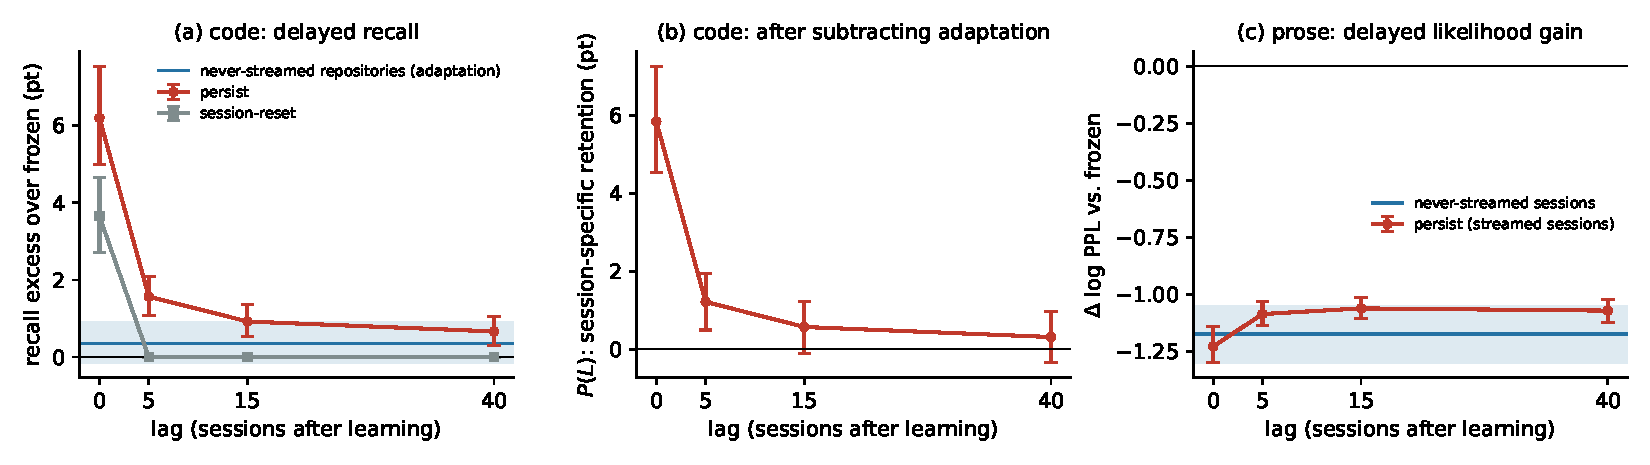
\includegraphics[width=\linewidth]{figs/fig1_identification.pdf}
\caption{Delayed recall against the never-streamed control (Qwen3-1.7B; session-clustered 95\% intervals). (a) Code: first-mention recall excess over the frozen model for persistent TTT and the session-reset control at lags 0--40 (3 seeds); the band is the excess of the final persist state on repositories never streamed. (b) The same data after subtracting the band, i.e.\ $P(L)$ of \S\ref{sec:estimand}; intervals combine both bootstraps. (c) Prose (3 seeds): likelihood gain on streamed sessions and on sessions never streamed.}
\label{fig:ident}\end{figure}

\subsection{Persistent TTT produces a strong short-lag effect}
At lag~0, persist reaches \persistAccZero\% first-mention recall against \baseAccZero\% for the frozen model (paired excess $\persistExcessLagZero\pt$, CI \persistExcessLagZeroCI; H1), a \foldLagZero$\times$ ratio; the likelihood gap is $\basePplZero\to\persistPplZero$ PPL (Fig.~\ref{fig:ident}). Per-document reset is indistinguishable from frozen (Table~\ref{tab:main}). Whatever persistence provides, it is provided across documents, not within them.

\subsection{The apparent memory tail}
The excess falls to $\persistExcessLagFive\pt$ at lag~5, $\persistExcessLagFifteen\pt$ at lag~15, and $\persistExcessLagForty\pt$ at lag~40 (CI \persistExcessLagFortyCI), still above frozen; H2 as stated is confirmed. Read on its own, this curve suggests a memory that decays quickly and then persists at a low level for at least forty sessions. That reading is the one a delayed-recall experiment invites, and it is the one we test next.

\subsection{The never-streamed control changes the interpretation}\label{sec:fresh}
The final persist state, scored on repositories that were never streamed, exceeds the frozen model by $\freshTransfer\pt$ (CI \freshTransferCI). This gain cannot be memory of any session; it is adaptation to the stream. It is of the same size as the lag-40 residual, and each interval contains the other's point estimate. On prose the same comparison is sharper: the lag-0 likelihood gain of $\eThreeStreamZero$ log-PPL is \eThreeShare\% matched by never-streamed sessions ($\eThreeFresh$, CI \eThreeFreshCI). We therefore do not treat the long-lag result as evidence for session-specific memory. H2 holds in the form in which it was stated; what changed is what it measures. Fig.~\ref{fig:ident} shows the never-streamed level as a band; the persist curve enters it between lag~5 and lag~15.

\subsection{What remains: session-specific retention}
Subtracting stream adaptation (\S\ref{sec:estimand}) gives $P(0)=\memZero\pt$, $P(5)=\memFive\pt$, $P(15)=\memFifteen\pt$ (CI \memFifteenCI), and $P(40)=\memForty\pt$ (CI \memFortyCI) on code; the last two intervals include zero. On prose, $P(L)$ includes zero at every lag. Session-specific retention is therefore real and large immediately after a session, falls by roughly four fifths within five sessions, and is not distinguishable from zero beyond fifteen. We do not conclude that it is absent; we conclude that our measurement cannot separate it from adaptation past that point. Lag-0 and lag-5 excess follow the same pattern at 0.6B and 4B (Fig.~\ref{fig:scale}a).

\begin{figure}[t]\centering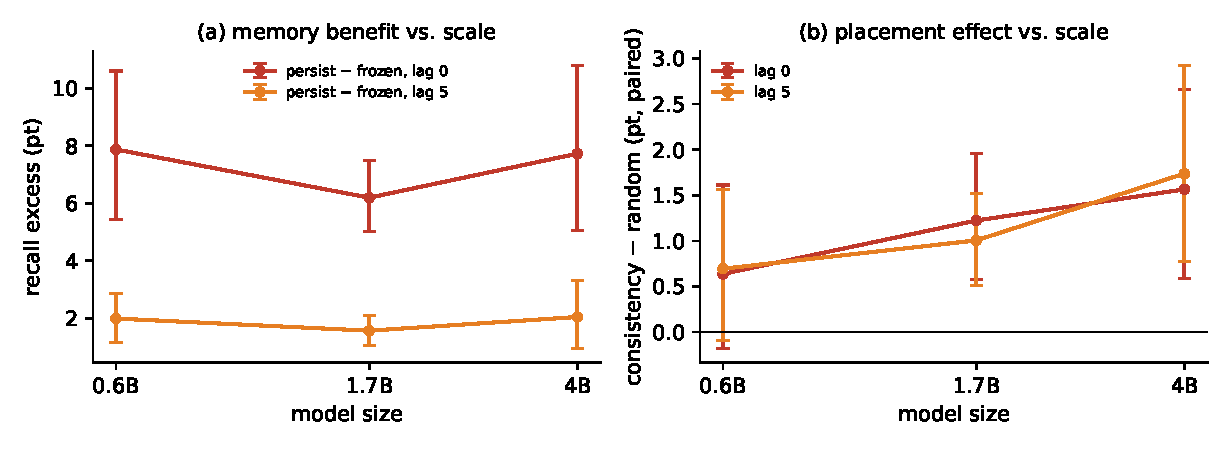
\includegraphics[width=.92\linewidth]{figs/fig3_scale.pdf}
\caption{Scale dependence (0.6B: 1 seed; 1.7B: 3 seeds; 4B: 1 seed; paired, clustered CIs). (a) Lag-0 excess is similar across scales. (b) Consistency $-$ random at equal budget grows with scale: $\crSmallZero$, $\crZero$, $\crLargeZero\pt$ at lag~0.}\label{fig:scale}\end{figure}

\subsection{Write load, not learning rate, predicts the decay}\label{sec:eta}
Prop.~\ref{prop:snr} was formulated before the learning-rate sweep and predicts that lag curves at different $\eta$ coincide once normalized by their lag-0 excess. At 0.6B, $\eta\in\{2,3,4\}\times10^{-2}$ give normalized lag-5 retention of $\normTwo$, $\normThree$, $\normFour$ (Fig.~\ref{fig:collapse}). The slight ordering is in the direction one would expect from clip saturation; we did not test this directly. This write-mass dependence is consistent with the palimpsest picture of \citet{parisi1986memory}.

\begin{figure}[t]\centering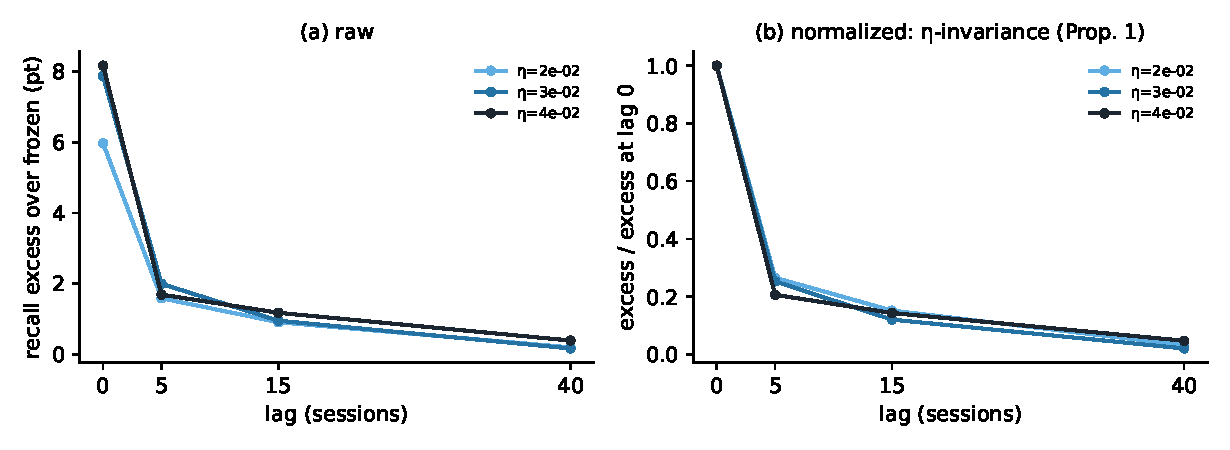
\includegraphics[width=0.85\linewidth]{figs/fig4_collapse.pdf}
\caption{Learning-rate invariance (0.6B, persist $-$ frozen). (a) Raw excess differs by $\eta$. (b) After normalizing by lag-0 excess the curves collapse, as Prop.~\ref{prop:snr} predicts.}\label{fig:collapse}\end{figure}

\subsection{Persistence has a capability cost}\label{sec:cost}
We use $\eta=3\times10^{-2}$, just below the capability cliff observed at 0.6B (between $3$ and $4\times10^{-2}$ the mean HellaSwag/ARC-Easy delta drops from $+0.9$ to $-6.9\pt$; 500 items per task). Even below that point, persistent policies at 1.7B lose $\taxHSRaw\pt$ on HellaSwag \citep{zellers2019hellaswag} and $\taxPIQARaw\pt$ on PIQA \citep{bisk2020piqa} under raw accuracy, and the same under length normalization (Fig.~\ref{fig:tax}a). ARC-Easy \citep{clark2018arc} moves $+\taxARCENorm\pt$ under length normalization but only $\taxARCERaw\pt$ in raw accuracy: the adaptation reshapes per-token likelihood in a way the normalized rule rewards without changing which answers are correct. We report both rules. At 4B the HellaSwag cost is comparable (Fig.~\ref{fig:tax}b; single seed).

\begin{figure}[t]\centering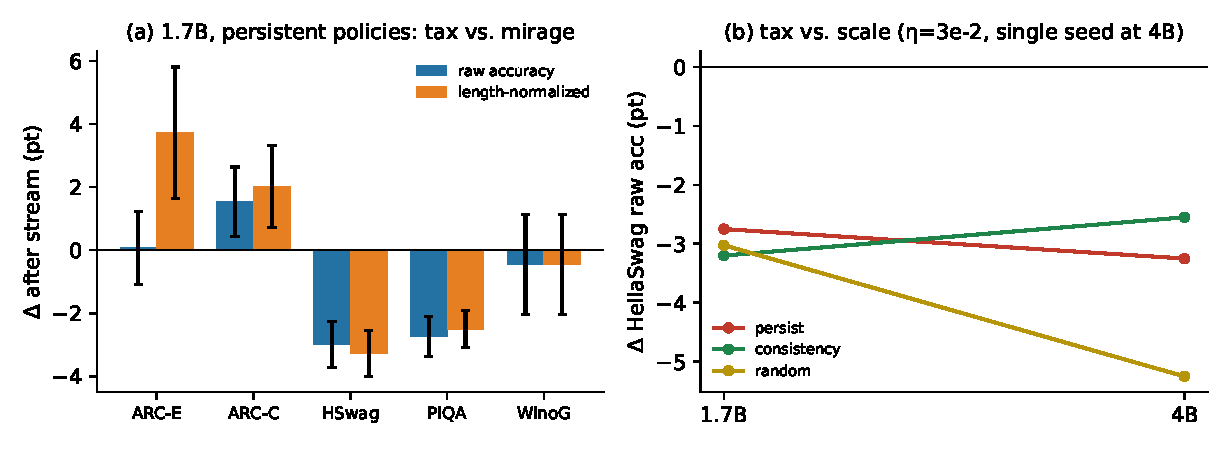
\includegraphics[width=0.85\linewidth]{figs/fig5_tax.pdf}
\caption{General-capability cost (a) and its scale dependence (b). At 1.7B, HellaSwag and PIQA losses appear under both scoring rules; the ARC-Easy gain under length normalization is a scoring artifact (raw accuracy is flat).}\label{fig:tax}\end{figure}

\subsection{Session-level reset as an operating point}
Session keeps \sessionCapture\% (\sessionCaptureMin--\sessionCaptureMax\% across seeds) of persist's lag-0 excess in recall and \sessionLogCapture\% in log-likelihood, has no cross-session exposure (Remark~\ref{rem:session}), and returns the model to its base state at stream end; within a session it carries the same exposure as persist. The paired persist advantage at lag~0 is $\spZero\pt$ (CI \spZeroCI; Fig.~\ref{fig:placement}b), of which stream adaptation explains $\freshTransfer\pt$; the remainder is not explained by our current controls. For the setting studied here, session reset keeps most of the short-lag benefit while avoiding the cost above and the cliff. Persistence adds two to three fast-weight-sized buffers and reduces throughput to $\approx0.4\times$ frozen inference; session needs no gate state.

\begin{figure}[t]\centering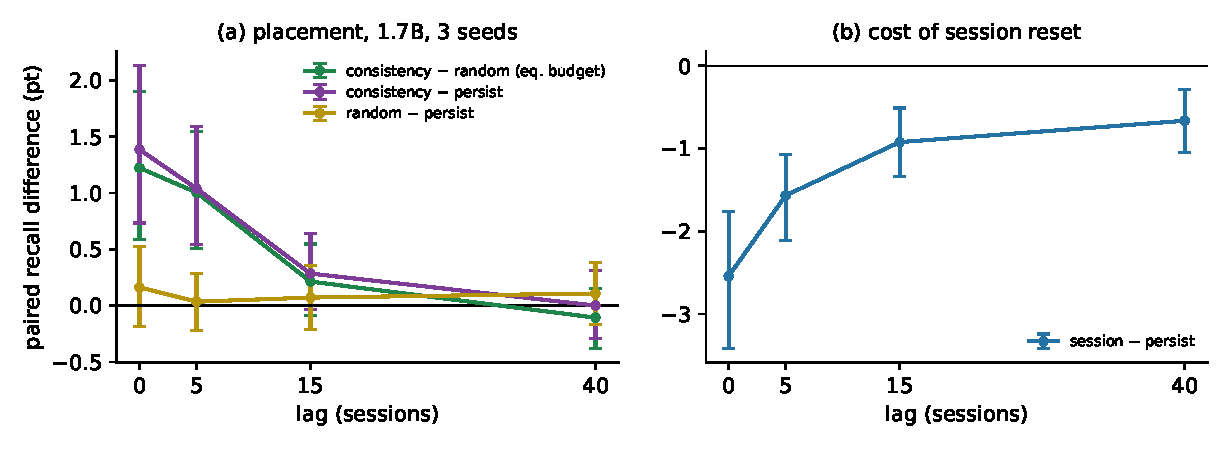
\includegraphics[width=0.85\linewidth]{figs/fig6_placement_E1.pdf}
\caption{Placement and the cost of reset (1.7B, 3 seeds, paired). (a) Consistency beats random at lags 0--5; random is indistinguishable from persist. (b) Session's deficit relative to persist shrinks from $\spZero$ to $\spForty\pt$.}\label{fig:placement}\end{figure}

\subsection{Selective writing improves short-lag recall, not the horizon}
At equal write budget, consistency gating beats random placement by $\crZero\pt$ at lag~0 (CI \crZeroCI) and $\crFive\pt$ at lag~5, and not beyond; random is indistinguishable from persist throughout. The difference is significantly nonzero (CI excludes zero) but lies within the prespecified $\pm2\pt$ equivalence margin, so H3 as stated is not rejected at 1.7B. It is absent at 0.6B and larger at 4B (Fig.~\ref{fig:scale}b; single seeds). On never-streamed repositories consistency and random tie, so on code the gate improves session-specific retention rather than adaptation; on prose it improves adaptation instead (App.~\ref{app:extra}), as Prop.~\ref{prop:gate} would predict for a gate that keeps whatever recurs. Decay, Fisher, and surprise gates are in App.~\ref{app:extra}.

\begin{table}[t]\centering\small
\caption{Main results (Qwen3-1.7B, 180 repositories, 3 seeds). Recall in \% with session-clustered 95\% CI; first-token PPL. $^\dagger$Equal write budget. \nHoldout\ held-out documents per seed, \nXfileTargets\ first-mention targets.}\label{tab:main}
\begin{tabular}{l cccc cccc}\toprule
& \multicolumn{4}{c}{recall (\%) at lag} & \multicolumn{4}{c}{PPL at lag}\\
policy & 0 & 5 & 15 & 40 & 0 & 5 & 15 & 40\\\midrule
frozen & 0.9 {\scriptsize[0.7,1.2]} & 1.0 {\scriptsize[0.7,1.2]} & 1.0 {\scriptsize[0.7,1.3]} & 1.0 {\scriptsize[0.7,1.3]} & 3510 & 3437 & 3451 & 3556 \\
persist & 7.1 {\scriptsize[6.0,8.4]} & 2.5 {\scriptsize[2.0,3.0]} & 1.9 {\scriptsize[1.6,2.3]} & 1.7 {\scriptsize[1.3,2.2]} & 398 & 678 & 825 & 934 \\
session-reset & 4.6 {\scriptsize[3.7,5.5]} & 1.0 {\scriptsize[0.7,1.2]} & 1.0 {\scriptsize[0.7,1.3]} & 1.0 {\scriptsize[0.7,1.3]} & 1229 & 3437 & 3451 & 3556 \\
consistency$^\dagger$\ & 8.5 {\scriptsize[7.2,10.0]} & 3.6 {\scriptsize[2.9,4.3]} & 2.2 {\scriptsize[1.8,2.6]} & 1.7 {\scriptsize[1.3,2.2]} & 358 & 578 & 747 & 873 \\
random$^\dagger$ & 7.3 {\scriptsize[6.1,8.6]} & 2.6 {\scriptsize[2.1,3.0]} & 2.0 {\scriptsize[1.6,2.4]} & 1.8 {\scriptsize[1.4,2.2]} & 401 & 669 & 823 & 925 \\
\bottomrule\end{tabular}\end{table}

\section{Discussion}\label{sec:discussion}

\textbf{What the experiments establish.} Under the controls of \S\ref{sec:protocol}, removing the document-boundary reset produces a large, session-specific gain immediately after a session ($P(0)=\memZero\pt$) that falls by about four fifths within five sessions and is still detectable at lag~5 ($P(5)=\memFive\pt$, CI \memFiveCI). The decay is predicted by subsequent write mass rather than learning rate, as Prop.~\ref{prop:snr} anticipated before the sweep was run. Unrestricted persistence costs $2$--$3\pt$ on two commonsense benchmarks under both scoring rules, and one length-normalized benchmark rises without any change in raw accuracy. At equal write budget, gating by sign consistency shifts a small amount of recall into short lags on code and into adaptation on prose.

\textbf{What they do not establish.} They do not show that session-specific memory is absent beyond fifteen sessions; they show that our measurement cannot separate it from stream adaptation there ($P(15)$ and $P(40)$ include zero). They do not show that delayed recall is uninformative in general, only that in this setting it did not identify persistence without the never-streamed control. The linear model reproduces the decay's dependence on write mass under isotropy that the benchmark itself induces; natural streams are not isotropic, and we have not tested the collapse on them. The residual persist--session gap at lag~0 ($\spZero\pt$) is not explained by our current controls; faster within-session learning from a warm-started state is one candidate we have not isolated.

\textbf{Practical implication.} For training-free fast-weight TTT of the kind studied here, resetting at session boundaries keeps most of the short-lag benefit, returns the model to its base state at stream end, and avoids the learning-rate cliff. Persisting across sessions buys a further $\spZero\pt$ at lag~0 and a residual that we cannot attribute, at a measurable capability cost. Which side of that trade is right depends on the deployment; we would not persist across sessions by default.

\textbf{Limitations.} The fresh-session control has 65 repositories (\nFresh\ with qualifying held-out files) and 28 prose sessions, and its intervals are correspondingly wide. Three seeds at 1.7B were the largest replication we could afford on a single A100; 0.6B and 4B are single-seed, so the size dependence in Fig.~\ref{fig:scale} is a trend, not a scaling result. Our learning rate sits just below the capability cliff on code and was calibrated separately for prose; other streams will need their own calibration. Decay, Fisher, and surprise gates were compared only on the pre-fix stream (App.~\ref{app:extra}). Learned gates, replay, and TTT architectures trained for persistence are outside our scope. Persistent adaptation on user streams raises retention and privacy questions; session reset is also the conservative default there.

\section{Conclusion}
For the training-free, fast-weight TTT setting studied here, memory is local. Persistence helps within a session but decays with subsequent write load; what survives beyond 15 sessions cannot be distinguished from adaptation to the stream. Resetting at session boundaries captures most of the benefit without the benchmark cost or privacy exposure. The question for future work is how much write load a memory can survive before it is overwritten.

\subsection*{AI use statement}
We used a generative AI assistant (Claude, Anthropic) extensively as a research and engineering assistant. Its contributions included proposing and refining candidate hypotheses, suggesting experimental controls and protocol details, assisting with the synthetic-stream and obfuscation implementation, developing and checking drafts of the linear-interference model and its propositions, writing and editing code, generating figures from raw results, suggesting experimental parameters, drafting the manuscript, and identifying related work.

The authors determined the research question, central scientific argument, experimental objectives, and final interpretation of the results. In particular, the identification of session-specific persistence from the never-streamed control, the definition of the persistence estimand, and the conclusions drawn from the control experiments were determined by the authors based on the experimental evidence. AI-generated hypotheses, model formulations, proofs, and interpretations were treated as proposals rather than authoritative results.

All experiments were run by the authors. All reported numbers were regenerated from raw logs using scripts inspected by the authors. The authors take responsibility for the final scientific claims, analyses, code, figures, and manuscript.

\subsection*{Reproducibility statement}
Experimental code, stream construction scripts, obfuscation pipelines, and unit tests are provided as supplementary material. Hyperparameters are listed in App.~\ref{app:hparams}; all base checkpoints are public (Qwen3-0.6B/1.7B/4B-Base). Bootstrap seeds and stream orderings are included in the supplementary material. Evaluation uses the public lm-eval-harness with fixed few-shot seeds.

\subsection*{Ethics statement}
Persistent adaptation raises retention and privacy questions; we recommend session-reset as the privacy-conservative default. The code stream uses only MIT-licensed repositories; the repository list with licenses is included in the supplement. No human subjects were involved.

\bibliography{references}
\bibliographystyle{iclr2027_conference}

\appendix
\section{Proofs}\label{app:proofs}
\textbf{Setup.} $G\in\mathbb{R}^{d_{\mathrm{out}}\times d}$; sessions write $\Delta_1,\Delta_2,\dots$; $m_k=\lVert\Delta_k\rVert_F$. A1 (independence): $\{\Delta_j\}$ independent with $\mathbb{E}\Delta_j=0$ over vocabulary randomization. A2 (isotropy): a probe $v$ of session $k$ is a unit vector uniform on the sphere, independent of $\{\Delta_j\}_{j\ne k}$ (it may depend on $\Delta_k$).

\emph{Proof of Prop.~\ref{prop:snr}.} For $j\ne k$, $v$ is independent of $\Delta_j$ by A2, so $\mathbb{E}\lVert\Delta_jv\rVert^2=\mathrm{tr}(\mathbb{E}[\Delta_j^\top\Delta_j]\,\mathbb{E}[vv^\top])=m_j^2/d$; cross terms vanish by A1. Interference power at lag $L$ is $\sum_{j\ne k,\,j\le k+L}m_j^2/d$; with $c_k:=\lVert\Delta_kv\rVert/m_k\le1$ (Cauchy--Schwarz), $\mathrm{SNR}=\sqrt d\,c_km_k/\sqrt{\sum_{j\ne k,\,j\le k+L} m_j^2}$. $\square$ Recall accuracy is a monotone function of SNR under a fixed-margin readout; the collapse test uses only monotonicity. If $m_j=\eta t_j\kappa(\eta)$, $\rho$ is $\eta$-free whenever $\kappa$ is.

\emph{Proof of Prop.~\ref{prop:gate}.} $D_t=\gamma_dD_{t-1}+(1-\gamma_d)s_t$, $s_t$ i.i.d.\ $\pm1$, $P(+1)=p$. Stationarity gives $\mathbb{E}D=2p-1$, $\mathrm{Var}D=\frac{1-\gamma_d}{1+\gamma_d}(1-(2p-1)^2)$; $\mathbb{E}|D|\ge|\mathbb{E}D|$ (Jensen) with equality as $\mathrm{Var}\to0$. $\square$

\emph{Boundedness.} For gates with $\alpha\le1$: element-wise clipping by $m$ over $N$ parameters gives $\lVert\delta\rVert_F\le m\sqrt N$, hence $\lVert G\rVert_F\le m\sqrt N\,T$ after $T$ writes and $\le m\sqrt N\,T_s/(1-\gamma)$ under boundary decay $\gamma$. The equal-budget cap of $4\times$ scales the bound accordingly.

\emph{Remark~\ref{rem:session}.} Immediate from the definition: $G_{\mathrm{slow}}=0$ at the start of every session, so for any probe of session $k$ at lag $\ge1$ both signal and interference vanish; within a session the update sequence equals persist's.

\section{Streams}\label{app:streams}
\textbf{Code.} \nRepos\ MIT-licensed Python repositories created after 2025-06 (30--1500 stars), files in import-dependency order, at most 8192 tokens per file; module- and class-level definitions ($\ge3$ characters, non-dunder) renamed to random lowercase strings with a per-repository RNG. Held-out: the last file with $\ge5$ first-mention targets (\nHoldout/180 qualify). 65 further repositories (\nFresh\ with qualifying held-out files) are never streamed. \textbf{Prose.} WikiText-103 \citep{merity2017wikitext} articles ($\ge8$k characters) split into $\approx1200$-token documents (3--12 per session); recurring capitalized phrases renamed with a per-session substitution cipher; \nESessions\ stream sessions, 28 fresh. Tokenization: Qwen3 tokenizer; targets scored at the position predicting the first sub-token.

\section{Hyperparameters}\label{app:hparams}
Chunk 256, context 1024 within document, $\eta=m=3\times10^{-2}$ (code; calibrated to $10^{-2}$ on prose to match the tax), $\gamma_d=0.9$, gate normalization capped at $4\times$, all layers' down-projections, bf16. Models: Qwen3-0.6B/1.7B/4B-Base \citep{qwen3}. General capability: lm-eval-harness \citep{gao2023lmeval}, 2000 items per task, fixed few-shot seeds, raw and length-normalized accuracy both recorded.

\section{Leak-freedom tests}\label{app:leak}
Unit tests assert: (1) eval-only passes never mutate parameters; (2) each recorded chunk loss equals a frozen model holding the pre-write state; (3) reset equals processing documents in isolation; (4) persist $\equiv$ decay($\gamma{=}1$); (5) the random gate's histogram equals the consistency gate's exactly. Held-out documents are scored before any boundary transition at lag~0.

\section{Six artifacts}\label{app:caution}
(1) Pre-training contamination (38.1\%$\to$1.7\%). (2) In-context copying (repeat mentions $\approx$65\% vs.\ first mentions $\approx$1\% for frozen). (3) Shared synthetic vocabulary across sessions (Fig.~\ref{fig:vocab}). (4) Boundary ordering: scoring lag~0 after a session reset reads frozen. (5) Length-normalized scoring (Fig.~\ref{fig:tax}a). (6) Stream-level slot adaptation on prose (Fig.~\ref{fig:ident}c).

\begin{figure}[h]\centering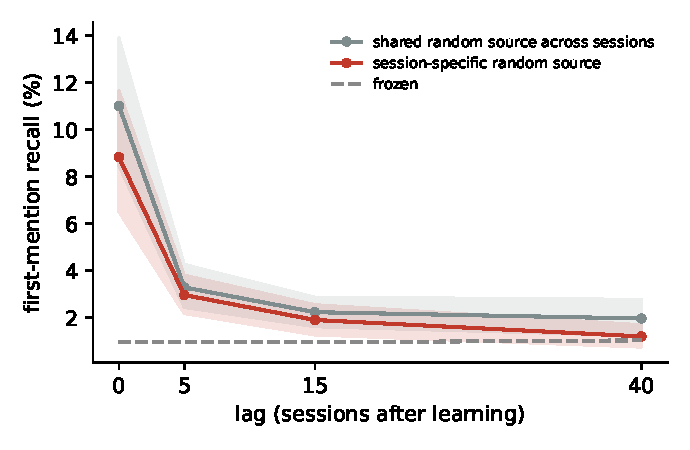
\includegraphics[width=0.5\linewidth]{figs/fig_vocab_artifact.pdf}
\caption{A shared random source for synthetic names across sessions (0.6B, pre-fix stream) inflates recall at every lag and roughly doubles it at lag~40; a session-specific source removes the effect. Frozen model dashed.}\label{fig:vocab}\end{figure}

\section{Additional policies}\label{app:extra}
Decay, Fisher, and surprise gates, and an activation-subspace projection (GPM-style, $k{=}64$; \citealp{saha2021gpm}), were evaluated at 0.6B on 50- and 200-repository streams \emph{before} the per-session-vocabulary fix (App.~\ref{app:caution}, item 3). Only their lag-0 ordering is therefore interpretable: all three gates were dominated by persist, and their apparent ``retention'' tracked how little they wrote; the projection halved lag-0 plasticity. Its apparent gain at lags 15--40 ($\approx0.5\pt$) lies within the shared-vocabulary inflation and is not claimed. The $6\times10^{-2}$ learning-rate point comes from the same pre-fix stream. Tables are in the supplement, labeled accordingly. On prose, consistency lowers log-PPL by $0.10$ relative to random at lag~0 (CI \eThreeCRZeroCI) and by a similar margin on never-streamed sessions ($\eThreeFreshCR$), so its advantage there is adaptation rather than session memory.

\section{Hypotheses fixed in advance}\label{app:prereg}
H1 confirmed. H2 confirmed as stated; interpretation revised by the fresh-session control (\S\ref{sec:fresh}). H3: equivalence within $\pm2\pt$ holds at 0.6B and 1.7B; at 4B the single-seed intervals (upper bounds $2.6$--$2.9\pt$) are too wide to establish it. A nonzero difference of about $1$--$1.7\pt$ at lags 0--5 is detected at 1.7B and 4B, and not at 0.6B. All other comparisons are exploratory.

\end{document}
